\documentclass[12pt]{article}
\usepackage[utf8]{inputenc}
\usepackage[spanish,activeacute]{babel}
\usepackage{amsmath}
\usepackage{geometry}
\usepackage{fancyhdr}
\usepackage{graphicx}
\usepackage{hyperref}
\hypersetup{
    colorlinks=true,
    linkcolor=blue,
    urlcolor=blue
}
\usepackage{xcolor}
\usepackage{enumitem}
\usepackage{framed}
\usepackage{tcolorbox}
\usepackage{draftwatermark} % Paquete para la marca de agua

% Configuración de la marca de agua
\SetWatermarkText{Analitiks Spa} % Texto de la marca de agua
\SetWatermarkScale{3} % Tamaño de la marca de agua
\SetWatermarkColor[gray]{0.9} % Color y transparencia de la marca de agua

% Configuración de márgenes
\geometry{left=2cm, right=2cm, top=2.5cm, bottom=2.5cm}

% Configuración del encabezado y pie de página
\pagestyle{fancy}
\fancyhf{}
\fancyhead[L]{
\includegraphics[width=2.5cm]{logo2.jpeg}}
\fancyhead[C]{\textbf{\sffamily Capstone Project: Analitiks Spa}}
\fancyfoot[C]{\thepage}

% Colores personalizados
\definecolor{primary}{RGB}{34, 85, 136}
\definecolor{secondary}{RGB}{0, 128, 128}
\definecolor{questionbg}{RGB}{240, 240, 240}

\begin{document}

% Título principal
\begin{center}
    \vspace*{8cm}
    {\Huge \textbf{\sffamily Informe de avance}}\\[0.5em]
\end{center}

\begin{center}
    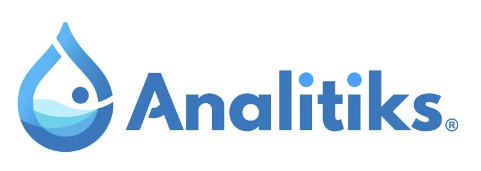
\includegraphics[width=8cm]{ANALITIKS.png}
\end{center}

\begin{center}
    \vspace{9cm}
    \textcolor{secondary}{\textbf{Santiago de Chile}}\\
    \textit{Viernes, 30 de septiembre de 2022}
    \vspace{1cm}
\end{center}


\newpage



% Índice
\tableofcontents
\newpage

% Resumen Ejecutivo
\section{Resumen Ejecutivo}

\subsection{Contexto}
Analitiks SpA es una empresa dedicada a la venta de instrumentos de medición de líquidos, enfocada principalmente en el sector minero pero con clientes en otros rubros como el de alimentos y la industria papelera. La dependencia de un pequeño grupo de clientes ha frenado su crecimiento, lo que ha motivado la necesidad de diversificar su cartera.

\subsection{Qué se hizo}
Se desarrolló una solución que unifica los datos de los clientes actuales y potenciales a través de una plataforma de unificación y análisis de datos. Se optimizaron los canales de captación, incluyendo automatización de procesos y análisis predictivo sobre datos históricos y actuales.

\subsection{Por qué y cómo se hizo}
Este proyecto se llevó a cabo para reducir la dependencia de pocos clientes, mejorar la identificación del cliente y aumentar la diversificación en un 30\% en 3 meses. Se utilizó una metodología ágil para el desarrollo iterativo, con ciclos de prueba y ajuste continuo.

\newpage

% Introducción
\section{Introducción}

\subsection{Contexto de la empresa}
\noindent
Analitiks SpA, fundada en agosto de 2019, se dedica a la venta y distribución de instrumentos de medición de líquidos, con un enfoque especializado en la entrega de soluciones para la medición y monitoreo en línea de fluidos. La empresa trabaja con una gama de instrumentos de alta calidad, fabricados principalmente en Alemania, garantizando precisión y fiabilidad en sus aplicaciones.\\
Entre los mercados principales en los que opera Analitiks se encuentran la minería, energía, pulpa y papel, y alimentos y bebidas. Estos sectores requieren soluciones robustas y precisas para asegurar la eficiencia en sus procesos productivos.
Analitiks SpA es el distribuidor oficial en Chile de reconocidas marcas internacionales, como Knick Elektronische Messgeräte GmbH \& Co. KG, SOPAT GmbH, Dr. Thiedig GmbH \& Co KG, Kuntze Instruments GmbH, EXNER Process Equipment GmbH, Real Tech Inc., Scentroid Inc., y Thermo Fisher Scientific, todas ellas líderes en sus respectivos campos.


\subsection{Contexto del problema}
\noindent
El principal reto ahora es diversificar la base de clientes, buscando oportunidades en sectores como el tratamiento de aguas y otras industrias. Esta expansión reduciría el riesgo de depender demasiado de un solo sector y abriría nuevas puertas para el crecimiento. Sin embargo, uno de los mayores obstáculos es la dificultad para atraer nuevos clientes, afectando las perspectivas de expansión. El síntoma más evidente es el lento ritmo en la adquisición de clientes nuevos, lo que impacta directamente en la sostenibilidad a largo plazo. Este problema genera un costo de oportunidad significativo al limitar la posibilidad de expansión a otros sectores. Las causas incluyen la falta de diversificación y desafíos en los canales de venta y distribución.
Resolver esta situación es crucial para desbloquear oportunidades de crecimiento y asegurar la competitividad. Para el equipo encargado, es una oportunidad de demostrar sus habilidades técnicas y de gestión dentro de la empresa.


\newpage

% Objetivos
\section{Objetivos}

\subsection{Objetivo General}
El objetivo principal de este proyecto es aumentar la diversificación de la cartera de clientes de Analitiks SpA en un 30\%, en un plazo de 3 meses, mediante la implementación de un sistema de gestión, análisis y segmentación de datos de clientes. Esta iniciativa permitirá a la empresa reducir su dependencia de un número limitado de clientes del sector minero, lo que ha sido un obstáculo para su crecimiento. Al diversificar su cartera, Analitiks podrá expandir su alcance a nuevos sectores industriales, como el tratamiento de agua, energía, y alimentos y bebidas, lo que permitirá un crecimiento sostenible y más equilibrado.
Para lograr este objetivo, se diseñará e implementará un sistema robusto de gestión de clientes (CRM), que unificará y centralizará todos los datos relevantes de clientes actuales y potenciales. Este sistema permitirá un análisis detallado de los patrones de compra, preferencias y comportamiento de los clientes, proporcionando a la empresa información clave para la toma de decisiones. Además, se desarrollarán estrategias personalizadas para cada segmento de clientes, con el fin de mejorar tanto la captación de nuevos clientes como la retención de los actuales.
Este proyecto no solo busca mejorar la diversificación, sino también optimizar la eficiencia operativa, al automatizar procesos de captación y análisis, y aumentar la personalización en las interacciones con los clientes. Al final del periodo de 3 meses, se espera que Analitiks cuente con una cartera de clientes más equilibrada y diversificada, que disminuya su vulnerabilidad frente a fluctuaciones del sector minero y aumente su competitividad en nuevos mercados.


\subsection{Objetivos específicos}
\subsubsection{Mejorar los indicadores que miden las preferencias de los actuales clientes.}
\noindent
El objetivo es desarrollar y refinar los mecanismos que permiten medir y analizar las preferencias de los clientes actuales y futuros de Analitiks SpA, para ofrecer soluciones más personalizadas y optimizadas. Al mejorar la medición de estas preferencias, Analitiks podrá ajustar su oferta de productos y servicios para adaptarse mejor a las necesidades específicas de cada cliente, aumentando su satisfacción y fidelidad. Los resultados de estas mediciones servirán también como base para estrategias de retención y crecimiento dentro de cada sector.
\subsubsection{Unificar los datos de clientes para analizar, predecir y accionar sobre clientes actuales y potenciales.}
\noindent
Unificar los datos dispersos de los clientes en una plataforma centralizada es crucial para obtener una visión integral y detallada de las interacciones, preferencias y patrones de comportamiento de los clientes. Este objetivo busca integrar datos provenientes de diferentes fuentes como el CRM, la página web, redes sociales y canales de comunicación directa, permitiendo un análisis predictivo más eficaz. Con esta unificación de datos, Analitiks podrá segmentar mejor su base de clientes, identificar oportunidades de ventas cruzadas, prever comportamientos futuros y accionar sobre las necesidades tanto de los clientes actuales como de los potenciales. Esta estrategia proporcionará una ventaja competitiva al permitir que las decisiones se basen en datos concretos y actualizados.
\subsubsection{Automatizar los canales existentes para optimizar la captación de clientes y el análisis de datos.}
\noindent
El objetivo de la automatización es mejorar la eficiencia en los procesos de captación y retención de clientes, utilizando herramientas que agilicen la interacción con los clientes y la recolección de datos. Esto incluirá la implementación de bots de atención al cliente, automatización de campañas de marketing y seguimiento automatizado de las interacciones a través de correo electrónico y redes sociales. La automatización permitirá a Analitiks responder de manera más rápida y eficiente a las consultas de los clientes, mientras recopila información valiosa que será utilizada para afinar las estrategias de captación y conversión. Además, optimizará el flujo de datos hacia el sistema centralizado, facilitando su análisis en tiempo real y mejorando la capacidad de reacción ante cambios en el comportamiento del cliente.


\subsection{Medidas de desempeño}
\subsubsection{Distribución de cartera de clientes}
\noindent
Medir el porcentaje de clientes diversificados por sector antes y después de la implementación del sistema es fundamental para evaluar el éxito de la estrategia de expansión hacia nuevos mercados. Este indicador analizará la distribución de clientes en sectores clave como minería, tratamiento de aguas, alimentos y bebidas. Se espera observar una mayor proporción de clientes en sectores no tradicionales, lo que indicará una diversificación efectiva. Esta métrica permitirá realizar un seguimiento preciso del progreso hacia la meta de diversificación del 30\% en tres meses. Los datos se recogerán mensualmente y se compararán con la línea base actual.
\subsubsection{Tasa de conversión}
\noindent
La tasa de conversión mide el número de clientes nuevos obtenidos a partir de las acciones de optimización de los canales de captación, como la página web, CDP y campañas de marketing automatizadas. Para lograr un análisis completo, se analizará la tasa de conversión de cada canal de captación por separado (e.g., página web, redes sociales, campañas de correo electrónico), permitiendo ajustar estrategias en tiempo real para maximizar la efectividad. La medición de la tasa de conversión se realizará de forma continua, y los resultados se revisarán mensualmente para evaluar el impacto de las optimizaciones y ajustes implementados en los canales.
\subsubsection{Recuperación de clientes}
\noindent
Medir el número de clientes que fueron recuperados tras la implementación de estrategias de re-engagement es crucial para evaluar la efectividad de las campañas dirigidas a clientes inactivos. Estas estrategias incluyen el uso de datos unificados para ofrecer promociones personalizadas, reactivación a través de correos electrónicos y llamadas de seguimiento. Este indicador permitirá medir el éxito de las campañas en términos de retención y lealtad de clientes, impactando directamente en la estabilidad de la base de clientes de la empresa. El seguimiento se realizará trimestralmente y se comparará con períodos anteriores para evaluar el retorno de inversión en las campañas de re-engagement.


\newpage

% Estado del arte
\section{Estado del Arte}

\subsection{Marco teórico}
\noindent
Hoy en día, las empresas que buscan diversificar su cartera de clientes y expandir su alcance utilizan Customer Data Platforms, que se centran en la unificación, recolección y análisis de datos. Las CDP integran y centralizan información de diversas fuentes, como interacciones en la página web, redes sociales, transacciones y puntos de contacto físicos, en una única plataforma. Esto permite construir perfiles de clientes detallados y unificados, proporcionando una visión integral y en tiempo real de cada cliente. 
En la literatura, Earley (2018) destaca que el uso de plataformas de datos de clientes, es crucial para integrar y analizar datos de múltiples fuentes, lo cual ofrece una visión integral de los clientes. Este enfoque permite a las empresas no solo entender mejor a sus clientes actuales, sino también identificar oportunidades para capturar nuevos segmentos. Por otro lado, Kabir (2016) enfatiza la importancia de los métodos sistemáticos de recolección de datos, destacando que la precisión y la consistencia en la captura de datos son esenciales para obtener información confiable que sustente decisiones estratégicas.

\subsection{Resolución del problema en la industria y literatura}
\noindent
La implementación de plataformas digitales integradas y el análisis predictivo se presentan como prácticas comunes y efectivas en la industria para aumentar la diversificación de clientes. Según Earley (2018), estas plataformas permiten a las empresas unificar fuentes de datos en un sistema central, facilitando la personalización de las estrategias comerciales. Al contar con información detallada y en tiempo real de cada cliente, las empresas pueden diseñar campañas específicas y recomendaciones personalizadas que resultan en una mayor captación y retención de clientes.
Los estudios de la industria y la literatura muestran que la adopción de herramientas de análisis predictivo en conjunto con las CDP es fundamental para anticipar las necesidades y comportamientos de los clientes. Un ejemplo de esta práctica es el uso de algoritmos basados en datos históricos recolectados y unificados en la CDP, los cuales predicen patrones de compra y preferencias, ayudando a las empresas a segmentar mejor sus mercados y diseñar ofertas que respondan de forma precisa a las necesidades de cada segmento.

\subsection{Herramientas y Métodos}
\subsubsection{Customer Data Platforms (CDP)}
\noindent
Los CDP son sistemas de gestión de datos que unifican información de clientes de múltiples fuentes, como CRM, redes sociales, interacciones en la página web y transacciones. Estas plataformas permiten a las empresas construir perfiles de clientes detallados y unificados, que se actualizan en tiempo real. Los CDP facilitan el análisis predictivo, la segmentación de clientes y la personalización de las estrategias de marketing y ventas. Al integrar datos dispersos en una única plataforma, las empresas pueden obtener una visión integral de sus clientes y tomar decisiones basadas en datos concretos y actualizados.

\subsubsection{Análisis Predictivo}
\noindent
El análisis predictivo es una técnica que utiliza datos históricos y actuales para predecir comportamientos futuros y tendencias. Al aplicar algoritmos y modelos matemáticos a los datos recolectados en la CDP, las empresas pueden anticipar las necesidades y preferencias de los clientes, segmentar mercados de forma más precisa y diseñar estrategias personalizadas. El análisis predictivo permite a las empresas tomar decisiones informadas y proactivas, en lugar de reactivas, lo que resulta en una mayor eficacia en la captación y retención de clientes.

\subsubsection{Integración y Minería de Datos}
\noindent
La integración y minería de datos son procesos clave para la unificación y análisis de datos en la CDP. La integración de datos de múltiples fuentes, como CRM, redes sociales y transacciones, permite a las empresas construir perfiles de clientes detallados y actualizados. La minería de datos consiste en extraer información valiosa y patrones ocultos de los datos recolectados, lo que facilita la identificación de tendencias y oportunidades de mercado. Estos procesos son fundamentales para la toma de decisiones basadas en datos y la personalización de las estrategias comerciales.

\subsection{Soluciones Factibles para Analitiks SPA}
\subsubsection{Implementación de una Customer Data Platform (CDP)}
\noindent
La implementación de un CDP que unifique todas las fuentes de datos de la empresa. Esta plataforma permitirá centralizar y estructurar la información recopilada en tiempo real, creando un repositorio de datos robusto que facilite el análisis de patrones y la toma de decisiones informadas sobre la diversificación de clientes. Según Earley (2018), las CDP son esenciales para lograr una integración eficiente de datos, optimizando así el uso de información operativa y de clientes.

\subsubsection{Integración de fuentes de datos en tiempo real}
\noindent
La integración de fuentes de datos en tiempo real mediante la conexión de sistemas y sensores que recopilan información de maquinaria y operaciones. Este enfoque permitirá a Analitiks recolectar datos críticos sobre el uso y rendimiento de su maquinaria en distintos sectores, identificando oportunidades para adaptar su oferta y explorar nuevos mercados.

\subsubsection{Desarrollo de un sistema de análisis predictivo enfocado en el comportamiento operativo y de mercado}
\noindent
Este sistema, en conjunto con la CDP, permitirá analizar datos históricos y en tiempo real para anticipar tendencias y evaluar la viabilidad de ingresar a nuevos segmentos de mercado, ajustando así las estrategias de diversificación de manera proactiva.

\subsection{Criterios para Elegir la Solución Propuesta}
\subsubsection{Unificación de Datos}
\noindent
Priorizar la integración y centralización de todas las fuentes de información de clientes en un único sistema permite a la empresa tener una visión integral de su base de clientes, lo que es esencial para personalizar las estrategias de marketing y alcanzar nuevos segmentos.

\subsubsection{Mejora de Canales Digitales}
\noindent
Dado que los canales digitales son una vía primaria de interacción con los clientes potenciales, se propone una mejora significativa de la página web y otras plataformas digitales para capturar datos relevantes de manera eficiente y en tiempo real.

\subsubsection{Facilidad de Implementación y Escalabilidad}
\noindent
Las soluciones propuestas, como la implementación de un CDP y un sistema de análisis predictivo, no sólo son técnicamente viables sino que también pueden escalarse conforme la empresa crezca y diversifique su mercado.

\begin{center}
    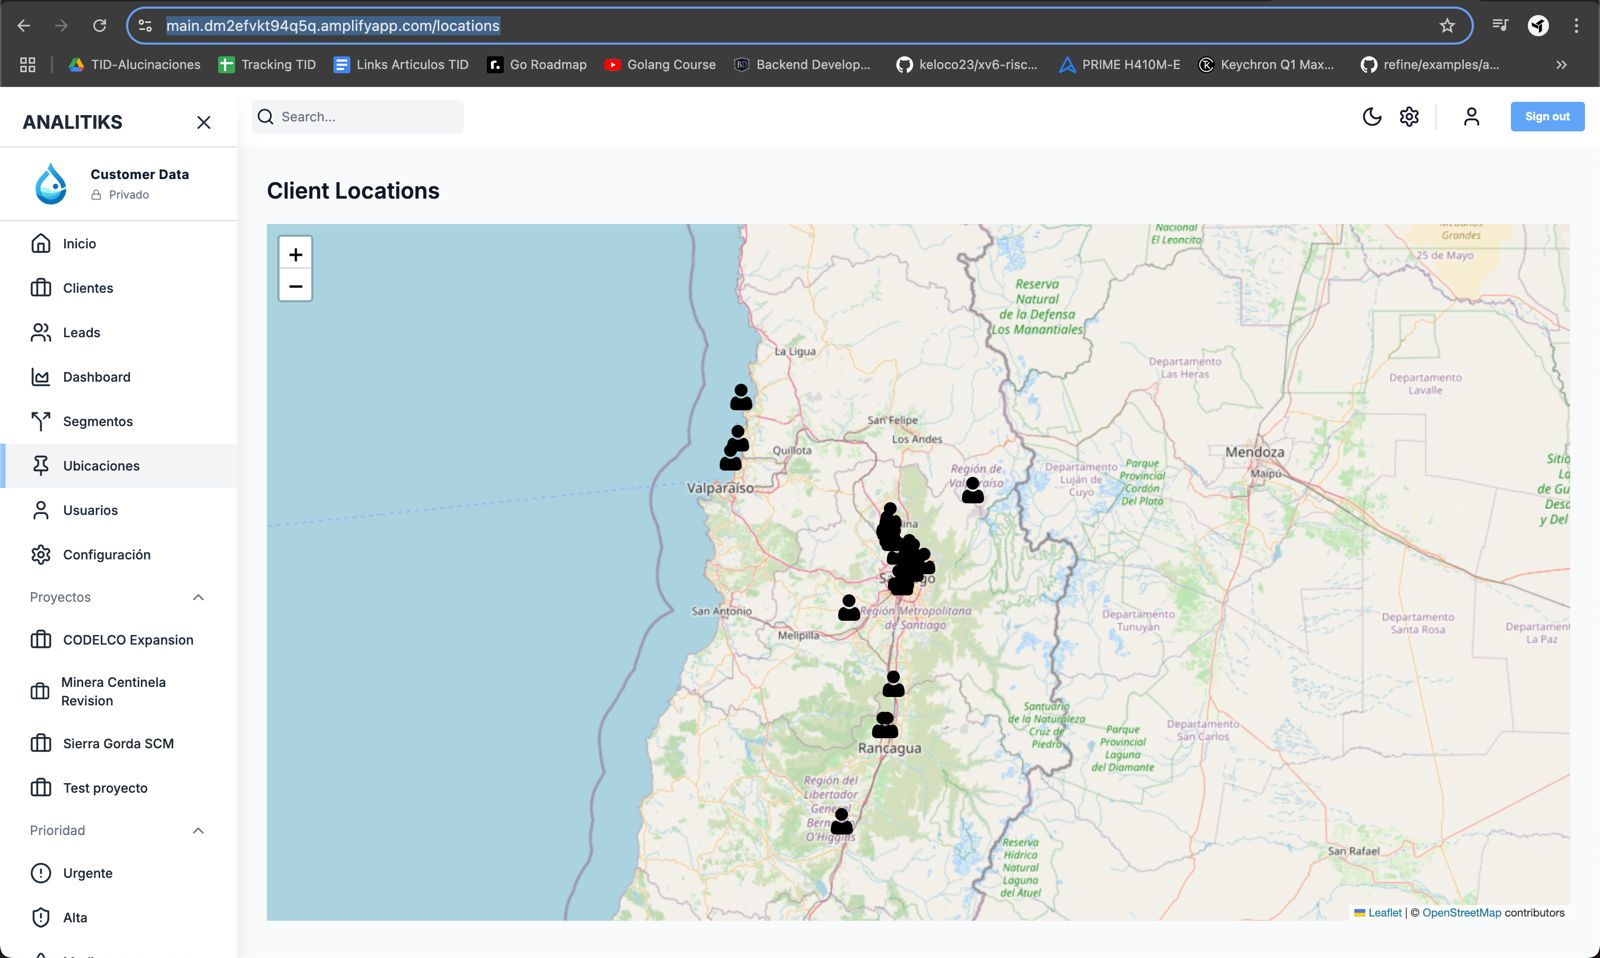
\includegraphics[width=19cm]{imagen33.jpeg}
\end{center}


\newpage

% Solución
\section{Solución}

\subsection{Metodologías}
\noindent
Se aplicará la metodología cascada/tradicional para la implementación del sistema de CDP y la mejora de la página web. Para el análisis de datos, se utilizará un enfoque de minería de datos y análisis predictivo. Se implementarán soluciones ya comprobadas que tienen un correcto funcionamiento para la captura de datos con herramientas para conectar las fuentes de información con nuestro CDP, como la API de Whatsapp, Linkedin y extracción de datos bruta a partir del CRM de la empresa, tomando un enfoque en la profundización de la información que se tiene del cliente. Estos datos se unificaran para crear diferentes visualizaciones del dato para generar nuevas estrategias para el objetivo comercial de Analitiks.

\subsection{Etapas de la solución}
\begin{enumerate}
    \item Implementación de una Customer Data Platform.
    \item Creación del contenido y estrategia de los datos.
    \item Desarrollo de un bot de WhatsApp.
    \item Integración de una API para LinkedIn.
    \item Recolección y análisis de datos unificados.
\end{enumerate}

\subsection{Descripción de la solución alcanzada}
\noindent
La solución implementada se basa en la unificación de los datos de los clientes en una plataforma centralizada, específicamente un Customer Data Platform (CDP), que permite la creación de perfiles detallados a partir de diversas fuentes de datos. Esta plataforma integra los datos históricos de ventas provenientes del CRM con los nuevos leads que se captaron a través de canales como el bot de WhatsApp y LinkedIn, lo que facilita una visión completa y actualizada de cada cliente. Al consolidar toda esta información en un único sistema, se elimina la duplicidad de datos y se asegura la precisión, mejorando así la gestión y segmentación de la cartera de clientes.
Uno de los principales componentes de esta solución es la automatización de los canales de captación de leads. El bot de WhatsApp, junto con las interacciones en LinkedIn, está configurado para captar información de los posibles clientes de manera eficiente y sin intervención manual. Estos inputs son procesados automáticamente y se integran directamente en el CDP, agilizando el proceso de generación de nuevos contactos y aumentando la tasa de conversión de leads en clientes efectivos. Este enfoque no solo acelera el flujo de trabajo, sino que también asegura que el equipo comercial disponga de información actualizada y relevante en todo momento.
Adicionalmente, el análisis predictivo desempeña un rol clave en la personalización de los servicios que se ofrecen. La plataforma permite anticipar las necesidades de los clientes mediante algoritmos que analizan su comportamiento, historial de compras y preferencias. Esto facilita la recomendación de productos, servicios o promociones que se ajusten a las expectativas de cada cliente, mejorando la experiencia de usuario y aumentando la retención. La personalización se convierte, entonces, en una ventaja competitiva al proporcionar a los clientes una atención más ajustada a sus necesidades específicas.
Por último, la centralización de los datos y la automatización también permiten optimizar la eficiencia operativa. La eliminación de tareas repetitivas y la minimización de errores manuales en la gestión de datos permiten que el equipo se concentre en tareas de mayor valor estratégico, como la toma de decisiones basadas en datos precisos y la implementación de campañas más efectivas. Esto no solo mejora la productividad interna, sino que también contribuye a fortalecer las relaciones comerciales con los clientes mediante una mejor segmentación y un enfoque personalizado.




\newpage

% Resultados esperados
\section{Resultados esperados}
Antes de su implementación, se espera que la solución aumente en un 30\% la diversificación de la cartera de clientes, mejore la tasa de conversión en un 20\% y optimizar la retención de clientes en un 30\%.

% Referencias
\section{Referencias}
\begin{itemize}
    \item Earley, Seth. (2018). The Role of a Customer Data Platform. IT Professional. 20. 69-76. 10.1109/MITP.2018.011301803.
    \item Kabir, Syed Muhammad. (2016). METHODS OF DATA COLLECTION.
\end{itemize}

\end{document}
